%!  pour pdfLatex
\documentclass[a4paper]{article}
%\usepackage[hmargin={1.5cm,1.5cm},vmargin={2.4cm,2.4cm},headheight=13.1pt]{geometry}
\usepackage[a4paper,landscape,twocolumn,
            hmargin=1.8cm,vmargin=2.2cm,headheight=13.1pt]{geometry}

\usepackage[pdftex]{graphicx,color}
\usepackage[pdftex,colorlinks={true},urlcolor={blue},pdfauthor={remy Nicolai}]{hyperref}

\usepackage[T1]{fontenc}
\usepackage[utf8]{inputenc}

\usepackage{lmodern}
\usepackage[frenchb]{babel}

\usepackage{fancyhdr}
\pagestyle{fancy}

\usepackage{floatflt}
\usepackage{maths}

\usepackage{parcolumns}
\setlength{\parindent}{0pt}

\usepackage{caption}
\usepackage{subcaption}

\usepackage{makeidx}

\usepackage[french,ruled,vlined]{algorithm2e}
\SetKwComment{Comment}{\#}{}
\SetKwFor{Tq}{tant que}{}{}
\SetKwFor{Pour}{pour}{}{}
\DontPrintSemicolon
\SetAlgoLined

\usepackage{listings}
\lstset{language=Python,frame=single}
\lstset{literate=
  {á}{{\'a}}1 {é}{{\'e}}1 {í}{{\'i}}1 {ó}{{\'o}}1 {ú}{{\'u}}1
  {Á}{{\'A}}1 {É}{{\'E}}1 {Í}{{\'I}}1 {Ó}{{\'O}}1 {Ú}{{\'U}}1
  {à}{{\`a}}1 {è}{{\`e}}1 {ì}{{\`i}}1 {ò}{{\`o}}1 {ù}{{\`u}}1
  {À}{{\`A}}1 {È}{{\'E}}1 {Ì}{{\`I}}1 {Ò}{{\`O}}1 {Ù}{{\`U}}1
  {ä}{{\"a}}1 {ë}{{\"e}}1 {ï}{{\"i}}1 {ö}{{\"o}}1 {ü}{{\"u}}1
  {Ä}{{\"A}}1 {Ë}{{\"E}}1 {Ï}{{\"I}}1 {Ö}{{\"O}}1 {Ü}{{\"U}}1
  {â}{{\^a}}1 {ê}{{\^e}}1 {î}{{\^i}}1 {ô}{{\^o}}1 {û}{{\^u}}1
  {Â}{{\^A}}1 {Ê}{{\^E}}1 {Î}{{\^I}}1 {Ô}{{\^O}}1 {Û}{{\^U}}1
  {œ}{{\oe}}1 {Œ}{{\OE}}1 {æ}{{\ae}}1 {Æ}{{\AE}}1 {ß}{{\ss}}1
  {ű}{{\H{u}}}1 {Ű}{{\H{U}}}1 {ő}{{\H{o}}}1 {Ő}{{\H{O}}}1
  {ç}{{\c c}}1 {Ç}{{\c C}}1 {ø}{{\o}}1 {å}{{\r a}}1 {Å}{{\r A}}1
  {€}{{\euro}}1 {£}{{\pounds}}1 {«}{{\guillemotleft}}1
  {»}{{\guillemotright}}1 {ñ}{{\~n}}1 {Ñ}{{\~N}}1 {¿}{{?`}}1
}

%pr{\'e}sentation des compteurs de section, ...
\makeatletter
\renewcommand{\thesection}{\Roman{section}.}
\renewcommand{\thesubsection}{\arabic{subsection}.}
\renewcommand{\thesubsubsection}{\arabic{subsubsection}.}
\renewcommand{\labelenumii}{\theenumii.}
\makeatother


\newtheorem*{thm}{Théorème}
\newtheorem{thmn}{Théorème}
\newtheorem*{prop}{Proposition}
\newtheorem{propn}{Proposition}
\newtheorem*{pa}{Présentation axiomatique}
\newtheorem*{propdef}{Proposition - Définition}
\newtheorem*{lem}{Lemme}
\newtheorem{lemn}{Lemme}

\theoremstyle{definition}
\newtheorem*{defi}{Définition}
\newtheorem*{nota}{Notation}
\newtheorem*{exple}{Exemple}
\newtheorem*{exples}{Exemples}


\newenvironment{demo}{\renewcommand{\proofname}{Preuve}\begin{proof}}{\end{proof}}
%\renewcommand{\proofname}{Preuve} doit etre après le begin{document} pour fonctionner

\theoremstyle{remark}
\newtheorem*{rem}{Remarque}
\newtheorem*{rems}{Remarques}

%\usepackage{maths}
%\newcommand{\dbf}{\leftrightarrows}

%En tete et pied de page
\lhead{Informatique}
%\chead{Introduction aux systèmes informatiques}
\rhead{MPSI B Hoche}
\lfoot{\tiny{Cette création est mise à disposition selon le Contrat\\ Paternité-Partage des Conditions Initiales à l'Identique 2.0 France\\ disponible en ligne http://creativecommons.org/licenses/by-sa/2.0/fr/  
} 
\rfoot{\tiny{Rémy Nicolai \jobname \; \today } }
}
\makeindex

%En tete et pied de page
\lhead{Cours IPT}
\chead{Résolution numérique d'équations différentielles ordinaires}
\begin{document}
\section{\'Equations différentielles et schémas numériques.}
\subsection{\'Equations différentielles ordinaires}
Une équation différentielle \emph{ordinaire} est une équation \emph{fonctionnelle} dont l'inconnue est une fonction dérivable d'une seule variable réelle. On peut toujours présenter une telle équation sous la forme
\begin{equation}
  y' = F\circ y
  \label{gene}
\end{equation}
où $F$ est une fonction donnée définie dans un ensemble $\mathcal{D}$ et où la fonction inconnue $y$ prend ses valeurs dans l'espace de définition de $F$.\newline
Il existe d'autres types d'équations fonctionnelles, par exemple les \emph{équations intégrales} ou les \emph{équations aux dérivées partielles}. Les équations aux dérivées partielles sont aussi des équations différentielles mais dont les inconnues sont des fonctions de plusieurs variables.\newline
Par exemple, pour des fonctions $K$ et $h$ données, l'équation de Fredholm
\begin{equation}
  \int_{a}^{b}K(x,t)y(t)\,dt = h(x)
  \label{fredholm}
\end{equation}
de fonction inconnue $y$ est une équation intégrale.\newline
Pour $k$ réel donné, l'équation de la chaleur
\begin{displaymath}
  \frac{\partial T}{\partial t} = k\frac{\partial^2 T}{\partial^2 x}
  \label{chaleur}
\end{displaymath}
de fonction inconnue $T$ est une équation aux dérivées partielles.\newline
Les solutions d'une équation différentielle ordinaire sont toujours des fonctions d'une seule variable mais, pour certaines équations, elles peuvent prendre leurs valeurs dans un espace vectoriel. C'est pour cela que toutes les équations différentielles ordinaires peuvent se mettre théoriquement sous la forme indiquée au début.\newline
Par exemple, pour $l$ et $g$ réels strictement positifs fixés, l'équation du pendule
\begin{equation}
  l\theta'' + g \sin \theta = 0
  \label{pendule}
\end{equation}
de fonction inconnue $\theta$ à valeurs réelles se met sous la forme indiquée en considérant une fonction $F$ définie dans $\R^2$ par 
\begin{displaymath}
  F((u,v)) = (v,-\frac{g}{l}\sin u)
\end{displaymath}
Pour cette fonction $F$, une fonction $\theta$ est solution de l'équation du pendule \eqref{pendule} si et seulement si la fonction $t\mapsto (\theta(t),\theta'(t))$ est solution de l'équation différentielle sous la forme générale \eqref{gene}.

Exercice 1. Soit $f$ une fonction définie dans un intervalle $I$ de $\R$. Former une fonction $F$ définie dans $\R\times I$ et permettant de ramener le calcul des primitives de $f$ à celui des solutions de l'équation différentielle \eqref{gene} attachée à $F$.

Dans le cours de début d'année, on a étudié les équations différentielles du deuxième ordre à coefficients constants. Plus généralement, dans une équation différentielle d'ordre $p$, les fonctions inconnues sont à valeurs dans $\R$ (ou $\C$) et l'équation revient à une expression de la dérivée $p$-ième en fonction des autres dérivées.

Exercice 2. On considère l'équation
\begin{equation}
  y'' + 2y' - y = \ch
  \label{lin2}
\end{equation}
et la fonction $F$ définie dans $\R^3$ par:
\begin{displaymath}
  F((t,u,v)) = (1,v,-2v+u+\ch(t))
\end{displaymath}
Montrer que $f$ est solution de \eqref{lin2} si et seulement si $t\mapsto(t,f,f')$ est solution de \eqref{gene}.

Cet exemple permet de se convaincre que les équations différentielles d'un ordre quelconque dont les solutions sont des fonctions numériques peuvent se ramener à des équations de la forme générale dont les solutions sont à valeurs vectorielles.

\subsection{Déterminisme, espace des phases.}
Le premier résultat théorique relatif aux équations différentielles est le théorème de Cauchy-Lipschitz. Sous certaines conditions sur $F$ et $\mathcal{D}$, un réel $t_0$ et une valeur $v_0\in \mathcal{D}$ étant donnés, il existe un intervalle ouvert $I$ contenant $t_0$ et une solution $y$ de l'équation \eqref{gene} dans $I$ telle que $y(t_0)=v_0$.\newline
Ce résultat est à reformuler en termes déterministes. Pour une \emph{bonne} équation différentielle, une solution est complètement déterminée par des \emph{conditions initiales}.\newline
L'espace vectoriel contenant le domaine de définition $\mathcal{D}$ de la fonction $F$ caractérisant l'équation différentielle est appelé \emph{l'espace des phases}. Un point de $\mathcal{D}$ caractérise un \emph{état} du système modélisé par l'équation différentielle.\newline
Dans toute modélisation, l'ensemble des états du système est fondamental. On peut utiliser le terme \og espace des états\fg ~ pour récupérer l'intuition géométrique mais il ne faut pas le confondre avec l'espace physique contenant le système.\newline
Un exemple\footnote{tiré de \emph{\'Equations différentielles ordinaires} V. Arnold} d'espace des phases.\newline
Considérons deux villes $A$ et $B$ reliées par deux routes qui ne se croisent pas et deux véhicules, chacun sur sa route. Un état de ce système est un couple de positions des deux véhicules. Comme on peut repérer chaque véhicule par sa distance à la ville $A$ sur sa route, l'espace des phases est le rectangle $[0,l_1]\times[0,l_2]$ de $\R^2$ où $l_1$ et $l_2$ sont les longueurs des deux chemins.\newline
On suppose les routes assez proches l'une de l'autre pour que deux véhicules partant de $A$ et reliés par une ficelle de longueur légèrement inférieure à $2l$ puissent arriver en $B$ sans rompre la ficelle. La question qui nous intéresse est la suivante.\newline
Deux véhicules sphériques (rayon $l$) un partant de $A$ sur la première route, l'autre de $B$ peuvent-ils atteindre l'autre ville sans se heurter?\newline
En utilisant des courbes tracées sur l'espace des phases, argumenter pour justifier que ce n'est pas possible.

\subsection{Schémas numériques.}
L'étude mathématique des équations différentielles conduit à définir de nouvelles fonctions qui peuvent être considérées comme usuelles et à des algorithmes permettant, assez souvent, d'exprimer les solutions d'une équation différentielle à l'aide de ces nouvelles fonctions usuelles. Ces méthodes, qui conduisent à des expressions exactes, relèvent du calcul formel et ne figurent pas au programme de la classe.\newline
L'approche numérique du calcul des solutions utilise des \emph{schémas numériques}. Un schéma numérique est constitué par un système fini d'équations obtenues en remplaçant les fonctions par des suites de valeurs prises sur les points d'un \emph{maillage} et la dérivation par un \emph{opérateur discret} sur ces suites de valeurs. Il s'agit d'obtenir ainsi une approximation de la solution pour une certaine condition initiale.
\subsubsection{Méthode d'Euler - Schéma numérique d'Euler.}
L'équation considérée\footnote{On se ramène à la forme générale en considérant les fonctions $t\mapsto (t,y(t))$.} ici est de la forme
\begin{equation}
  y'(t) = F((t,y(t)))
  \label{euler}
\end{equation}
où $F$ est une fonction définie dans une partie de $\R^2$ et à valeurs réelles. On cherche à approcher la solution qui vaut $y_0$ en $a$.
\begin{itemize}
  \item Le maillage est obtenu à partir d'un  \emph{pas} $h$ : on pose $t_k = a + kh$.
  \item On remplace la fonction par des valeurs $y_k$ associées aux points $t_k$.
  \item On remplace la dérivation par l'opérateur discret 
  \begin{align*}
  f &\mapsto f'\\
(y_0,y_1,\cdots,y_k,\cdots)&\mapsto \left(\frac{1}{h}(y_1-y_0), \frac{1}{h}(y_2-y_1),\cdots, \frac{1}{h}(y_{k+1}-y_k),\cdots \right)      
  \end{align*}
\end{itemize}
On aboutit ainsi à un système d'équations aux inconnues $y_1,y_2,\cdots$
\begin{align*}
  &y_1 = y_0 + hF(t_0,y_0) \\ &y_2 = y_1 + hF(t_1,y_1)\\ &\vdots \\ &y_{k+1} = y_k + hF(t_k,y_k)
\end{align*}
qui admet clairement une unique solution qui se calcule facilement.

\subsubsection{Variante - Schéma d'ordre 2.}
On se place dans les mêmes conditions que dans le paragraphe précédent sauf que l'on change l'opérateur discret en utilisant $\frac{1}{2h}(y_{k+1}-y_{k-1})$ au lieu de $\frac{1}{h}(y_{k+1}-y_{k})$ pour $k\geq 2$. On aboutit à un autre système d'équations
\begin{align*}
  &y_1 = y_0 + hF(t_0,y_0) \\ &y_2 = y_0 + 2hF(t_1,y_1)\\ &y_3 = y_1 + 2hF(t_2,y_2)\\ &\vdots \\ &y_{k+1} = y_{k-1} + 2hF(t_k,y_k)
\end{align*}

\subsubsection{Problématique de la validité}
\emph{Convergence du schéma}. Pour un pas $h$ fixé, on peut considérer
\begin{displaymath}
  \varepsilon(h)=\max_{k}|y(t_k) - y_k|
\end{displaymath}
Le schéma est dit convergent lorsque la fonction $\varepsilon$ converge vers $0$ en $0$.\newline
\emph{Consistance du schéma}. La consistance d'un schéma est liée à la validité de l'opérateur discret comme approchant la dérivation.\newline
Montrer que pour une fonction de classe $\mathcal{C}^3$ sur un segment $I$,
\begin{displaymath}
  \left|\frac{1}{h}\left( f(t_{k+1})-f(t_k)\right) -f'(t_k) \right|\leq h\frac{M_2}{2},\hspace{0.5cm}
  \left|\frac{1}{2h}\left( f(t_{k+1})-f(t_{k-1}\right) -f'(t_k) \right|\leq h^2\frac{M_3}{2}
\end{displaymath}
où $M_2 = \max_{I}|f"|$ et $M_3 = \max_{I}|f^{(3)}|$. L'exposant $2$ du $h$ justifie la dénomination ordre $2$ dans la variante. La consistance est meilleure dans le schéma d'ordre $2$, mais cela ne suffit pas forcément à améliorer la convergence.\newline
\emph{Stabilité du schéma}. Comment varie le $y_k$ en fonction d'une petite variation du $y_0$?

\section{Implémentations de la méthode d'Euler}
On implémente la méthode d'Euler pour l'équation \eqref{euler} d'abord en pseudo code dans l'algorithme \ref{resolnumeqdiff_1}. 
\begin{algorithm}[h]
  \Donnees{\;
    $F$ la fonction de deux variables caractérisant l'équation différentielle\;
    $a$ et $b$ float: définissant l'intervalle sur lequel on cherche les solutions\;
    $h$ float: le pas \;
    $y_0$ float : la valeur intiale en $a$\;
  }
  \Comment{initialisation}
  $l_t\leftarrow [a]$ : liste des $t_k$\;
  $l_y\leftarrow [y_0]$ : liste des $y_k$\;
  $y\leftarrow y_0$: valeur courante \;
  $t\leftarrow a$: temps courant \;
  \Tq{ $t+h \leq b$}{
    $y \leftarrow y + hF(t,y)$\;
    Placer $y$ à la fin de $l_y$\;
    $t\leftarrow t +h$\;
    Placer $t$ à la fin de $l_t$\;
  }
  Renvoyer $l_t , l_y$\;
  \caption{Pseudo code pour la méthode d'Euler}
  \label{resolnumeqdiff_1}
\end{algorithm}
On l'implémente ensuite en python et on teste pour l'équation
\begin{equation}
  y' - \tau y =0
  \label{eqtau}
\end{equation}
avec $\tau$ réel fixé (égal à $1$) dont on cherche la solution dans l'intervalle $[0,1]$.
\lstinputlisting[firstline=7, lastline=29]{resolnumeqdiff1.py}

Exercice 3. Implémenter en Python la variante du schéma d'ordre $2$. La tester pour l'équation \eqref{eqtau} en formant les graphes de la solution et des deux familles de points obtenues pour les deux schémas avec un pas de $0.05$ dans les cas $\tau=1$ et $\tau=-3.5$.

\section{\'Equation du pendule.}
On se propose cette fois de mettre en oeuvre la méthode d'Euler pour l'équation du pendule. Dans ce cas, les solutions sont à valeurs dans un espace des phases de dimension $2$. En changeant les unités, on se ramène au cas où $\frac{g}{l}=1$. 
\lstinputlisting[firstline=7, lastline=32]{resolnumeqdiff2.py}
Interpréter les courbes de l'espace des phases obtenues par le code du dessus.
\begin{figure}[h]
  \centering
  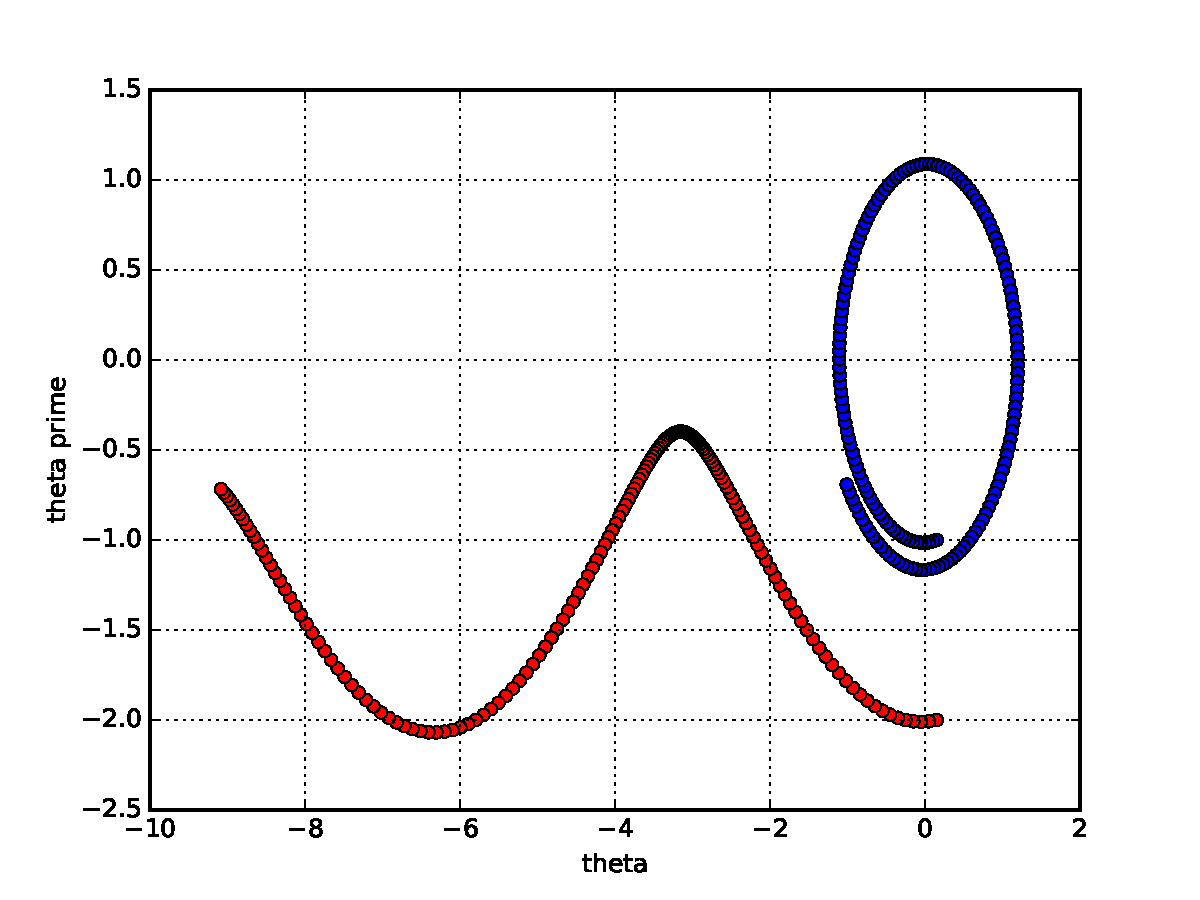
\includegraphics[width=10cm]{./resolnumeqdiff_1.pdf}
  % resolnumeqdiff_1.pdf: 576x432 pixel, 72dpi, 20.32x15.24 cm, bb=0 0 576 432
  \caption{Courbes de l'espace des phases}
  \label{fig:resolnumeqdiff_1}
\end{figure}
Ce genre de graphique s'appelle un portrait de phase. Quel est l'effet d'un changement d'unité sur un portrait de phases?

\section{Solution exercice 3}
\lstinputlisting[firstline=31, lastline=60]{resolnumeqdiff1.py}

\end{document}